\chapter{Architecture}
\label{chapter:arch}
\section{Overview}
In this chapter the overview of proposed system extension design will be discussed.
The proposed system was designed using top-down approach. First the user interface with regards to usability and Docker ecosystem, then the program managing the simulation and ways of communication with user interface that are most suitable for system usecases. Finally, the methods of connecting existing simulation programs with the managing program, and how to share data between them.
\section{User interface}
At very top of the system the top there is the user, that needs some interface to interact with the system.. The current interface to each component is CLI that is not suited for non-technical user, so there is a strong inclination to build a graphical interface. The two main kinds are native application with GUI and WEB-GUI. Thought the GUI of operating system inside of a docker container can be shared to host through VPNCS server or Xauthority, it is much easier to host simple http server that exposes a port to host, and can be accessed through web browser. For this reason, WEB-GUI interface was chosen as the preferred method of interacting with user. This part of the proposed will be refereed in this thesis as SimBaD-Client. This first design iteration can be visible on the figure \ref{fig:arch0}. It is important to underline that single component on diagram does not necessarily equal single docker container.
\begin{figure}[h!]
	\centering
		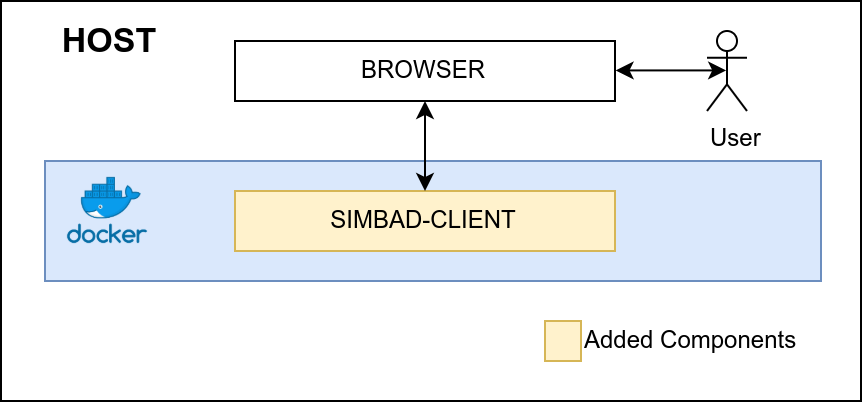
\includegraphics[width=0.9\linewidth]{diagrams/arch1.png}
	\caption{Architecture Overview: SimBaD Client}
	\label{fig:arch0}
\end{figure}
\section{Managing the simulation}
Another component that is necessary is a component that will connect all of the simulation pipeline steps together. This component should receive and execute commands from SimBad-Client. The use of web client narrows the possible methods of communications to network protocols and forces the component that receives commands to have web capabilities - to be a web server. Such component in this this will be referred to as SimBaD-Pipeline-Server. 
\subsection{Methods of communication}
There are several methods on server-client communications to choose from, in the following section the WebSocket, HTTP RPC and Graphql will be discussed.

WebSocket is a communication protocol that provides full-duplex (data can be send both ways at the same time) communication over TCP connection. From client standpoint it provides server push capabilities - client can receive updates from server without explicitly asking for them. This makes it more suitable for real-time communication. Because WebSockets reuse single TCP connection, they have very low overhead - after initial handshake there is no need to send such data as request headers or cookies. This also leads to very high throughput. 

The REST (Representational State Transfer) is an style of software architecture for creating web services. Rest puts some constraints such as  on a HTTP communication protocol. Using REST it is possible to define communication endpoint (an exposed interface) and operations, (usually CRUD) that can be made using that endpoint. The major benefit of REST is it allows to define very transparent interfaces. REST is a mature technology, and as such, it is very standardized with such standards as OpenApi and that helps with development and documentation. REST is most suitable when client-server interactions are less frequent. One of the principles of REST architecture is client-server split - REST defines a contract that both side of communication need to keep, thus allowing separate development of client and server. The obvious disadvantage of this approach is that it does not allow for real-time data to be passed to client. When clients needs to have updates from server, it has to continuously ask for it - such process is also called long polling. Operations can be defined as precisely as needed, but they nevertheless they need to be defined - it is common to get whole object to get information about its property which causes unnecessary data to be send, and to get only this property, separate endpoint needs to be defined. Such problem is also called over-fetching. The REST also suffers from the opposite of under-fetching, where to get necessary the client needs to make more than one request.

GraphQL or Graph Query Language, was developed by Facebook, to address the under-fetching and over-fetching issues without without writing additional endpoints.  It is a relatively new technology, as the specification of it was open-sourced in 2015. From client side it allows to define a structure of required data and from server side it allows to return specified data. In contrast to REST, where the structure of the response is defined by endpoint, in Graphql the structure of response is created by GraphQL engine to mach the structure of query. It supports the usual read/write CRUD operations using mutations along with real-time data updates using subscriptions. The downside of this solution is that is a s it is relatively new, its ecosystem and tools are fewer and less mature compared to REST. It is less suitable for simple APIs as it adds a lot of complexity.

To chose one, it is necessary to analyze the needs of the system for sending data. The user should trigger simulation by sending configuration file, and this would be the main case where the system needs to handle user input. After that, the client needs to get update from server about simulation progress - this would be the most common operation. Because the simulation can go on a very long time, there's no need for frequent updates, as changes to simulation state occur rarely. When simulation step or simulation as a whole finishes, user needs to be able to view and download its results. The WebSocket does not really add anything of value to the system, as data does not need to be real time, the updates are rare, and keeping single connection open for several days is not something one should do.  REST API is suited for above use-cases, and due to its standardization and tooling its the easiest one to develop with. The GraphQL API while promising, is a slight overkill for such simple system, as the problems that it solves are not as common, however, this solution will become more viable with system grow. In conclusion, the REST API was chosen as preferred communication between system components. 
\begin{figure}[h!]
	\centering
		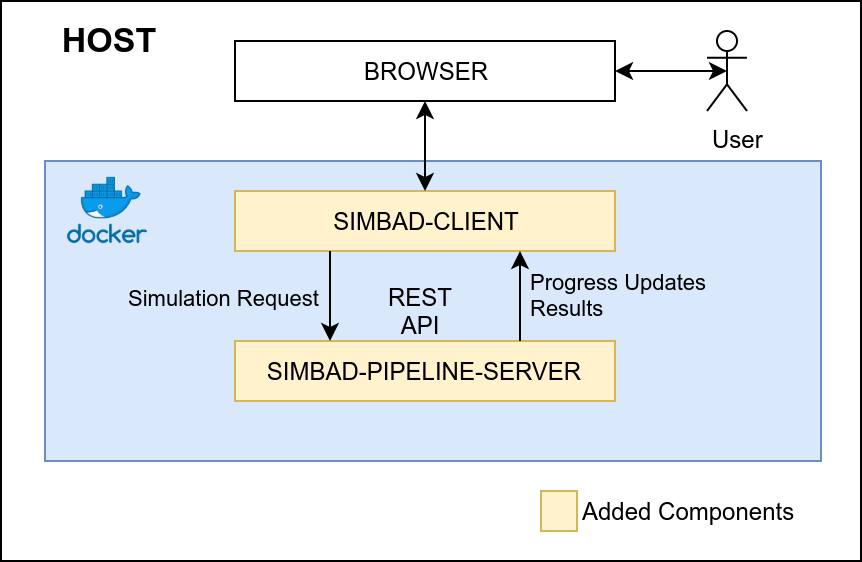
\includegraphics[width=0.9\linewidth]{diagrams/arch2.png}
	\caption{Architecture Overview: Client and server}
	\label{fig:arch2}
\end{figure}
\newpage 
\subsection{API definitions}
All of the API interfaces defined in proposed system, were defined using the OpenApi standard. An example of such definition for operation that starts simulation process is visible on listing \ref{list:openapi-route}. OpenApi definition consist of route, operations allowed on this route, in this case "POST" operation, the request data and possible server responses - data and HTTP codes. Such definition defines a contract that both sides client and server must keep. To help with development, OpenApi allows to generate server and client code from such definition, which considerably speeds up the development process and prototyping. With code generator, using few commands one can generate client API code, server and mock server endpoints, and as long as the contract is kept, both sides of can be developed independent of each other.. The endpoints defined using this standard are very well documented, and easy to use for developers. Additional tools such as swagger editor can be used to create and visualize those definitions. 

\begin{lstlisting}[label=list:openapi-route,caption=The OpenAPI route definition for simulation start, basicstyle=\footnotesize\ttfamily]
paths:
  /api/simulation/start:
    post:
      tags:
        - SIMULATION
      operationId: startSimulation
      description: Starts simulation process
      requestBody:
        content:
          application:/json:
            schema:
              $ref: "#/components/schemas/StartSimulationRequest"
      responses:
        "202":
          description: Request is accepted and command starts to execute
          content:
            application/json:
              schema:
                $ref: "#/components/schemas/SimulationStepInfo"
        "400":
          description: Simulation process is already running
          content:
            application/json:
              schema:
                $ref: "#/components/schemas/SimulationError"
components:
  schemas:
    StartSimulationRequest:
      type: object
      properties:
        configurationName:
          description: The configuration file name
          type: string
        configuration:
          description: The configuration file to be sent to CLI
          type: string
          format: binary
      required:
        - configuration
        - configurationName
\end{lstlisting}
\subsubsection{Sharing and persisting data}
The first step of devising a proper way to share data for such pipeline system is to figure out how data should be passed between components. In its current state, the components do not pass whole files directly to each other, but rather pass the paths to files. The consequence of this is that each component needs to have access to filesystem where the file resides, and this in turn poses a question: how to give access to the same filesystem to multiple separate components? Docker solves such problem using Docker volumes.  Though the data in container can also be stored in the top read-write layer, such data is deleted when container is deleted. Docker volumes are a way to persist and share data between containers or between containers and host. The program running inside of container sees such volume as a folder, and can write and read data to it. Same volume can be used by multiple docker containers, solving the problem of shared filesystem. Apart from existence of actual simulation data on the filesystem, some kind of additional metadata should be specified - such information as the path to output file or which file is the result of which simulation or step. Though such information can also be stored in the filesystem, for example in some kind of .csv or .json file, it is more convenient to store them in database. As the writes and reads to the database are sparse, and the data written is of small size, SQlite database was chosen. The data in Sqlite database is stored in single .sqlite file, that can also be stored on the shared volume. This choice also reduces the docker footprint on system, as other databases like MySql or Postgress would require separate container, over 100MB in size.
\begin{figure}[h!]
	\centering
		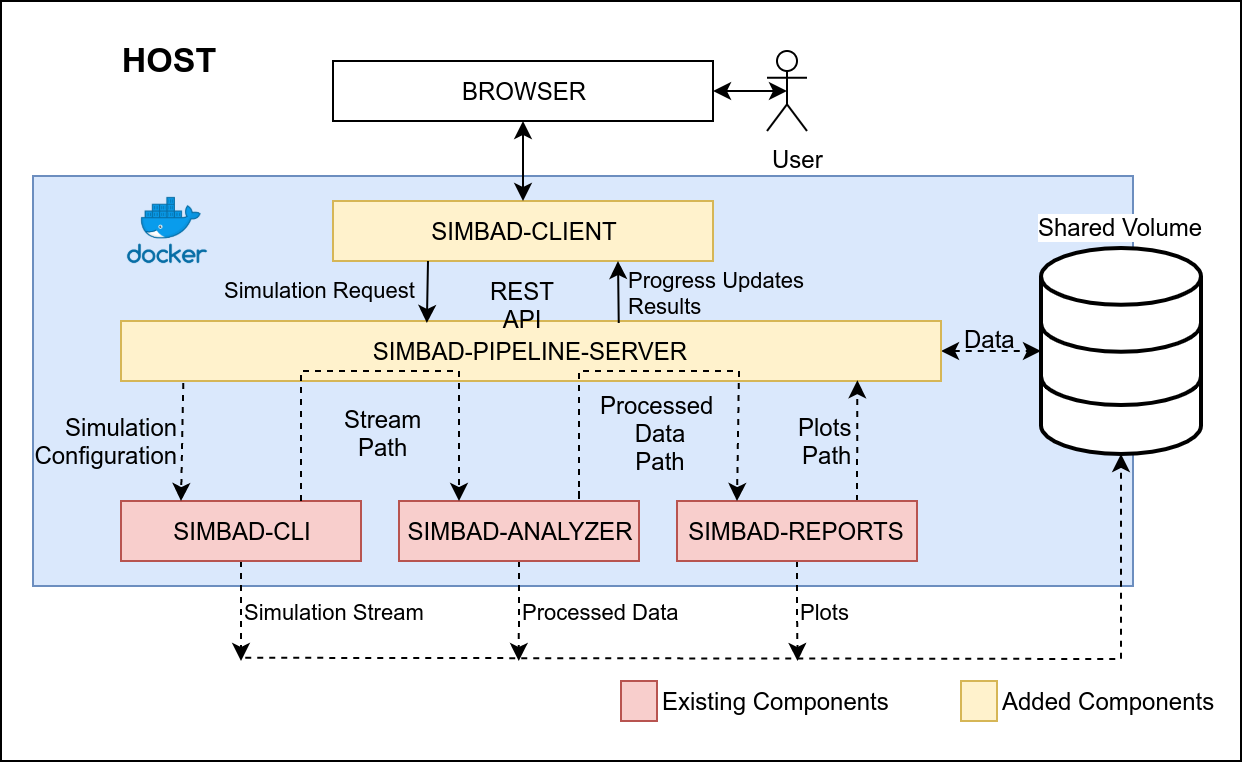
\includegraphics[width=0.9\linewidth]{diagrams/arch4.png}
	\caption{Overview of system architecture}
	\label{fig:arch4}
\end{figure}
\section{Extending existing components}
The usual way to communicate between docker containers is to use networking. As existing components do not have networking capabilities, the only viable way to connect all of them is to place them in single container, so the pipeline server can issue command by directly executing components scripts and binaries. This however does not fulfill the modularity and configurability goals, because it prevents components from being decoupled and enforces single viable configuration. The components also should not be modified directly, as that would violate the non-invasive integration constraint. The solution that satisfies all that is to add simple http server on top of each component that should be able to independent. This layer should allow to trigger the execution, get the progress, and get the result of step. For the purpose of this thesis, such extension was added to SimBaD-Analyzer step. Through use of SSH tunnel forwarding, this extension can also function over SSH-only connections.
\section{Summary}
In the proposed architecture, the user will control and monitor the simulation process with web client - SimBaD-Client. The client, using HTTP RPC will issue commands to the server (SimBaD-Pipeline-Server), and the server will connect all of the simulation components together and manage simulation process. To connect all of the simulation steps to server, two methods will be used: storing simulation step scripts and binaries on the same container as server, or for separate containers, adding HTTP RPC API on top of simulation step, without modifying it.